
\section{Similarities Between Functions}

Note that functions that are identical at the IR or machine level are not
necessarily identical at the source level.
Figure~\ref{fig:identical-example} shows two real functions extract from the
447.dealII program in the SPEC CPU2006~\cite{spec} benchmark suite.
Although these two functions are not identical at the source level, they become
identical after a template specialization and some optimizations are applied, in
particular, constant propagation, constant folding, and dead-code elimination. 
Specializing \verb|dim| to $1$ enables to completely remove the loop in the
function \verb|PolynomialSpace|.
Similarly, specializing \verb|dim| to $1$ results in only the first iteration
of the loop in the function \verb|TensorProductPolynomials| being executed.
The compiler is able to statically analyze and simiplify the loops in both
functions, resulting in the identical functions shown at the bottom of
Figure~\ref{fig:identical-example}.

\begin{figure}[h]
\centering
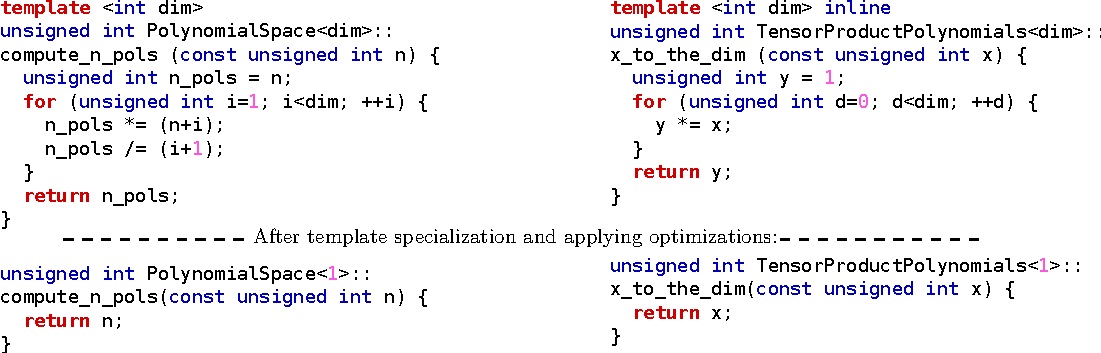
\includegraphics[width=\textwidth]{src/relatedwork/figs/identical-example}
\caption{Two function extracted from the 447.dealII benchmark that are not
           identical at the source level, but after applying template
           specialization and optimizations they become identical at the IR
           level.}
\label{fig:identical-example}
\end{figure}

\section{Identical Code Folding in Linkers}


Google developed an optimization for the \textit{gold} linker that merges
identical functions on a bit-level~\cite{tallam10,kwan12}.
After placing each function in a separate ELF section, they identify function
sections that have their \textit{text} section bit-identical and also their
relocations point to sections that are identical. A simpler version of this
optimization was also offered by the MSVC linker~\cite{msvc-icf};

\section{Identical Function Merging}


A similar optimization for merging identical functions, but instead at the
intermediate representation (IR) level, is also offered by both GCC and
LLVM~\cite{llvm-fm,livska14}.
%The function merging optimization currently offered by LLVM is only able to
%merge identical functions.
This optimization is only flexible enough to accommodate simple type mismatches
provided they can be bitcasted in a losslessly way.
%Similarly to the technique proposed by Edler von Koch~et~al.~\cite{edler14},
%LLVM's optimization also exploits structural similarity among functions.
%However, the current implementation does not allow instructions to differ in
%their opcodes or in the number and type of their input operands.
%Although very restrictive, this optimization guarantees that any pair of
%mergeable functions will result in code size reduction with no performance
%overhead.
%Its simplicity also benefits compilation time, as the actual merge operation
%is trivial.
Its simplicity allows for an efficient exploration approach based on computing
the hash of the functions and then using a tree to identify equivalent functions
based on their hash values.

